\documentclass[11pt,a4paper]{report}
\usepackage[textwidth=37em,vmargin=30mm]{geometry}
\usepackage{calc,xunicode,amsmath,amssymb,paralist,enumitem,tabu,booktabs,datetime2,xeCJK,xeCJKfntef,listings}
\usepackage{tocloft,fancyhdr,tcolorbox,xcolor,graphicx,eso-pic,xltxtra,xelatexemoji}

\newcommand{\envyear}[0]{2025}
\newcommand{\envdatestr}[0]{2025-05-31}
\newcommand{\envfinaldir}[0]{webdb/2025/20250531/final}

\usepackage[hidelinks]{hyperref}
\hypersetup{
    colorlinks=false,
    pdfpagemode=FullScreen,
    pdftitle={Web Digest - \envdatestr}
}

\setlength{\cftbeforechapskip}{10pt}
\renewcommand{\cftchapfont}{\rmfamily\bfseries\large\raggedright}
\setlength{\cftbeforesecskip}{2pt}
\renewcommand{\cftsecfont}{\sffamily\small\raggedright}

\setdefaultleftmargin{2em}{2em}{1em}{1em}{1em}{1em}

\usepackage{xeCJK,xeCJKfntef}
\xeCJKsetup{PunctStyle=plain,RubberPunctSkip=false,CJKglue=\strut\hskip 0pt plus 0.1em minus 0.05em,CJKecglue=\strut\hskip 0.22em plus 0.2em}
\XeTeXlinebreaklocale "zh"
\XeTeXlinebreakskip = 0pt


\setmainfont{Brygada 1918}
\setromanfont{Brygada 1918}
\setsansfont{IBM Plex Sans}
\setmonofont{JetBrains Mono NL}
\setCJKmainfont{Noto Serif CJK SC}
\setCJKromanfont{Noto Serif CJK SC}
\setCJKsansfont{Noto Sans CJK SC}
\setCJKmonofont{Noto Sans CJK SC}

\setlength{\parindent}{0pt}
\setlength{\parskip}{8pt}
\linespread{1.15}

\lstset{
	basicstyle=\ttfamily\footnotesize,
	numbersep=5pt,
	backgroundcolor=\color{black!5},
	showspaces=false,
	showstringspaces=false,
	showtabs=false,
	tabsize=2,
	captionpos=b,
	breaklines=true,
	breakatwhitespace=true,
	breakautoindent=true,
	linewidth=\textwidth
}






\newcommand{\coverpic}[2]{
    % argv: itemurl, authorname
    Cover photo by #2~~(\href{#1}{#1})
}
\newcommand{\makeheader}[0]{
    \begin{titlepage}
        % \newgeometry{hmargin=15mm,tmargin=21mm,bmargin=12mm}
        \begin{center}
            
            \rmfamily\scshape
            \fontspec{BaskervilleF}
            \fontspec{Old Standard}
            \fontsize{59pt}{70pt}\selectfont
            WEB\hfill DIGEST
            
            \vfill
            % \vskip 30pt
            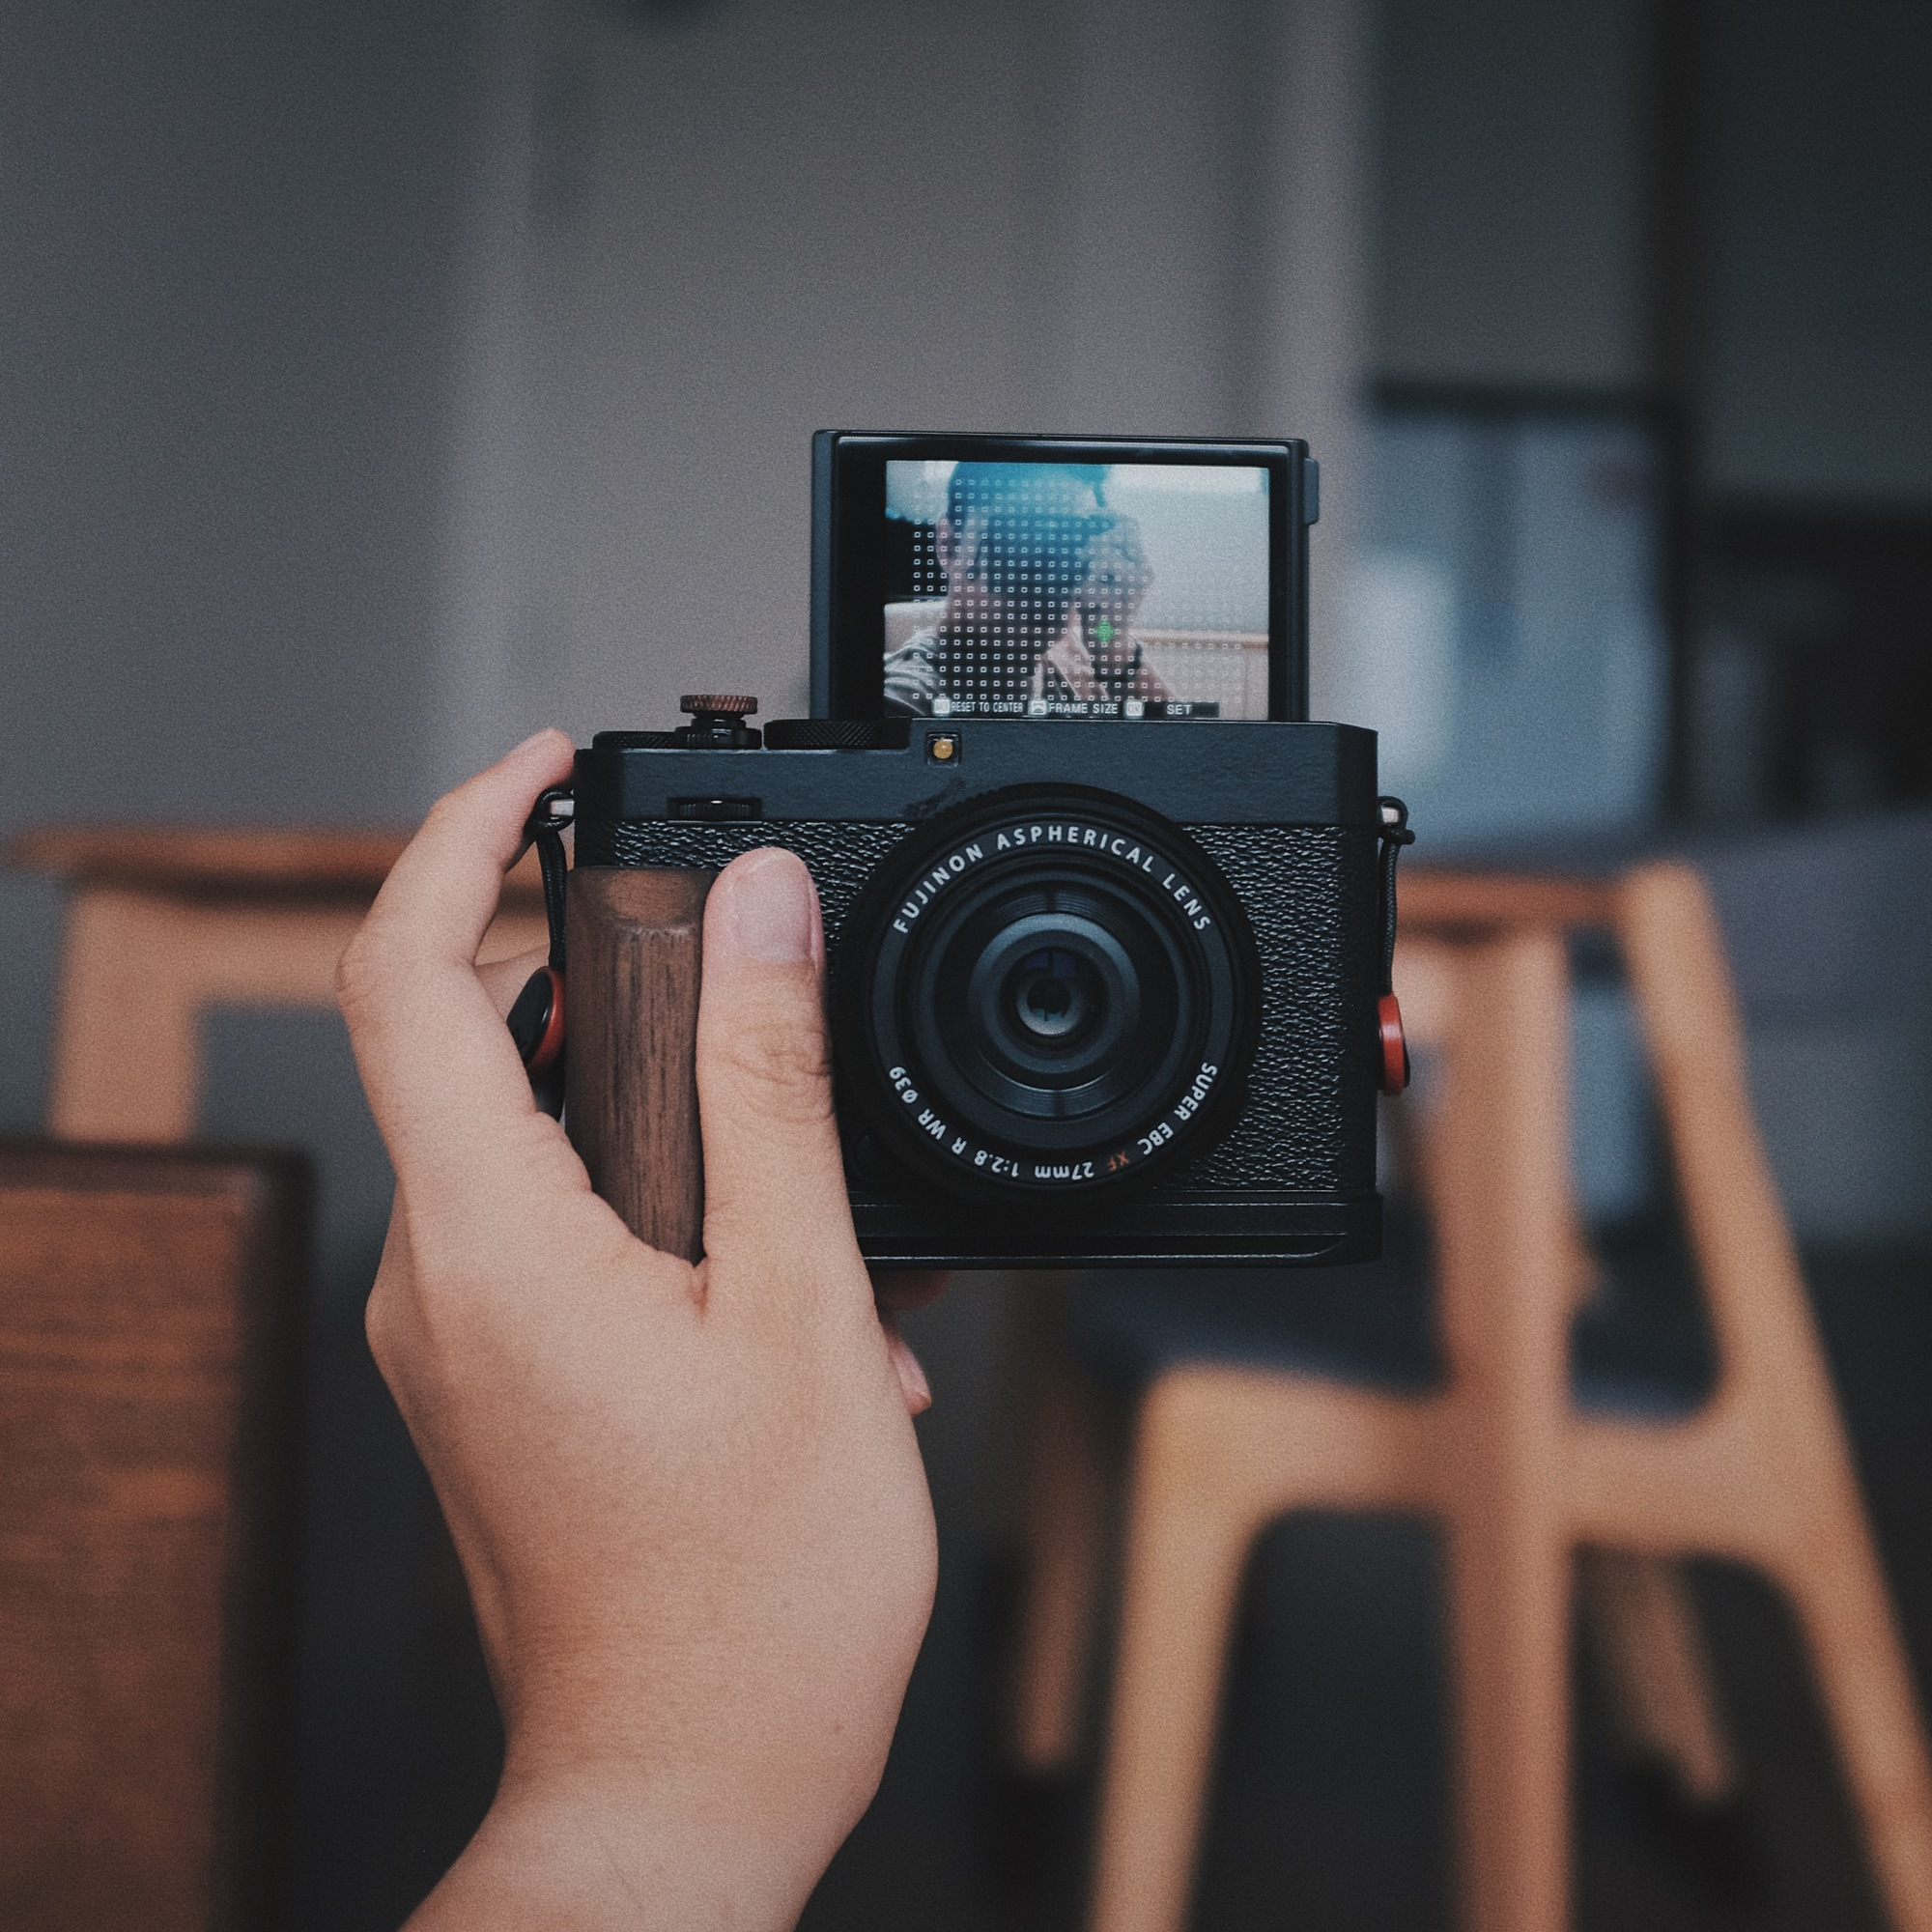
\includegraphics[width=\linewidth]{\envfinaldir/coverpic-prod.jpg}\par
            % \vskip 30pt
            \vfill

            \normalsize\rmfamily\scshape
            \copyright{} The Web Digest Project \hfill\large \envdatestr
        \end{center}
    \end{titlepage}
    % \restoregeometry
}
\newcommand{\simplehref}[1]{%
    \textcolor{blue!80!green}{\href{#1}{#1}}%
}
\renewcommand{\contentsname}{\center\Huge\sffamily\bfseries Contents\par\vskip 20pt}
\newcounter{ipartcounter}
\setcounter{ipartcounter}{0}
\newcommand{\ipart}[1]{
    % \vskip 20pt
    \clearpage
    \stepcounter{ipartcounter}
    \phantomsection
    \addcontentsline{toc}{chapter}{#1}
    % \begin{center}
    %     \Huge
    %     \sffamily\bfseries
    %     #1
    % \end{center}
    % \vskip 20pt plus 7pt
}
\newcounter{ichaptercounter}
\setcounter{ichaptercounter}{0}
\newcommand{\ichapter}[1]{
    % \vskip 20pt
    \clearpage
    \stepcounter{ichaptercounter}
    \phantomsection
    \addcontentsline{toc}{section}{\numberline{\arabic{ichaptercounter}}#1}
    \begin{center}
        \Huge
        \sffamily\bfseries
        #1
    \end{center}
    \vskip 20pt plus 7pt
}
\newcommand{\entrytitlefont}[1]{\subsection*{\raggedright\Large\sffamily\bfseries#1}}
\newcommand{\entryitemGeneric}[2]{
    % argv: title, url
    \parbox{\linewidth}{
        \entrytitlefont{#1}\par\vskip 5pt
        \footnotesize\ttfamily\mdseries
        \simplehref{#2}
    }\vskip 11pt plus 11pt minus 1pt
}
\newcommand{\entryitemGithub}[3]{
    % argv: title, url, desc
    \parbox{\linewidth}{
        \entrytitlefont{#1}\par\vskip 5pt
        \footnotesize\ttfamily\mdseries
        \simplehref{#2}\par\vskip 5pt
        \small\rmfamily\mdseries#3
    }\vskip 11pt plus 11pt minus 1pt
}
\newcommand{\entryitemAp}[3]{
    % argv: title, url, desc
    \parbox{\linewidth}{
        \entrytitlefont{#1}\par\vskip 5pt
        \footnotesize\ttfamily\mdseries
        \simplehref{#2}\par\vskip 5pt
        \small\rmfamily\mdseries#3
    }\vskip 11pt plus 11pt minus 1pt
}
\newcommand{\entryitemHackernews}[3]{
    % argv: title, hnurl, rawurl
    % \parbox{\linewidth}{
    %     \entrytitlefont{#1}\par\vskip 5pt
    %     \footnotesize\ttfamily\mdseries
    %     \simplehref{#3}\par
    %     \textcolor{black!50}{\href{#2}{#2}}
    % }\vskip 11pt plus 11pt minus 1pt
    \begin{minipage}{\linewidth}
            \entrytitlefont{#1}\par\vskip 5pt
            \footnotesize\ttfamily\mdseries
            \simplehref{#3}\par
            \textcolor{black!50}{\href{#2}{#2}}
    \end{minipage}\par\vskip 11pt plus 11pt minus 1pt
}







\begin{document}

\makeheader

\tableofcontents\clearpage




\ipart{Developers}
\ichapter{Hacker News}
\entryitemTwoLinks{Photos taken inside musical instruments}{https://news.ycombinator.com/item?id=44139626}{https://www.dpreview.com/photography/5400934096/probe-lenses-and-focus-stacking-the-secrets-to-incredible-photos-taken-inside-instruments}

\entryitemTwoLinks{Jerry Lewis's "The Day the Clown Cried" discovered in Sweden after 53 years}{https://news.ycombinator.com/item?id=44139592}{https://www.thenationalnews.com/arts-culture/film-tv/2025/05/29/jerry-lewis-day-the-clown-cried-discovered/}

\entryitemTwoLinks{Surprisingly Fast AI-Generated Kernels We Didn't Mean to Publish (Yet)}{https://news.ycombinator.com/item?id=44139454}{https://crfm.stanford.edu/2025/05/28/fast-kernels.html}

\entryitemTwoLinks{Cap: Lightweight, modern open-source CAPTCHA alternative using proof-of-work}{https://news.ycombinator.com/item?id=44137867}{https://capjs.js.org/}

\entryitemTwoLinks{Beating Google's kernelCTF PoW using AVX512}{https://news.ycombinator.com/item?id=44137715}{https://anemato.de/blog/kctf-vdf}

\entryitemTwoLinks{De Bruijn notation, and why it's useful}{https://news.ycombinator.com/item?id=44137439}{https://blueberrywren.dev/blog/debruijn-explanation/}

\entryitemTwoLinks{The 'white-collar bloodbath' is all part of the AI hype machine}{https://news.ycombinator.com/item?id=44136117}{https://www.cnn.com/2025/05/30/business/anthropic-amodei-ai-jobs-nightcap}

\entryitemTwoLinks{MinIO Removes Web UI Features from Community Version, Pushes Users to Paid Plans}{https://news.ycombinator.com/item?id=44136108}{https://biggo.com/news/202505261334\_MinIO\_Removes\_Web\_UI\_Features}

\entryitemTwoLinks{Microsandbox: Virtual Machines that feel and perform like containers}{https://news.ycombinator.com/item?id=44135977}{https://github.com/microsandbox/microsandbox}

\entryitemTwoLinks{Systems Correctness Practices at Amazon Web Services}{https://news.ycombinator.com/item?id=44135638}{https://cacm.acm.org/practice/systems-correctness-practices-at-amazon-web-services/}

\entryitemTwoLinks{The Darwin Gödel Machine: AI that improves itself by rewriting its own code}{https://news.ycombinator.com/item?id=44135369}{https://sakana.ai/dgm/}

\entryitemTwoLinks{Ask HN: What is the best LLM for consumer grade hardware?}{https://news.ycombinator.com/item?id=44134896}{https://news.ycombinator.com/item?id=44134896}

\entryitemTwoLinks{AI is not our future}{https://news.ycombinator.com/item?id=44134798}{https://procreate.com/ai}

\entryitemTwoLinks{Radio Astronomy Software Defined Radio (Rasdr)}{https://news.ycombinator.com/item?id=44134364}{https://radio-astronomy.org/rasdr}

\entryitemTwoLinks{RFK Jr's 'Maha' report found to contain citations to nonexistent studies}{https://news.ycombinator.com/item?id=44133962}{https://www.theguardian.com/us-news/2025/may/29/rfk-jr-maha-health-report-studies}

\entryitemTwoLinks{Buttplug MCP}{https://news.ycombinator.com/item?id=44133706}{https://github.com/ConAcademy/buttplug-mcp}

\entryitemTwoLinks{White House releases health report written by LLM, with hallucinated citations}{https://news.ycombinator.com/item?id=44132873}{https://www.nytimes.com/2025/05/29/well/maha-report-citations.html}

\entryitemTwoLinks{Show HN: MCP Server SDK in Bash}{https://news.ycombinator.com/item?id=44132823}{https://github.com/muthuishere/mcp-server-bash-sdk}

\entryitemTwoLinks{Triangle splatting: radiance fields represented by triangles}{https://news.ycombinator.com/item?id=44132744}{https://trianglesplatting.github.io/}

\entryitemTwoLinks{The radix 2^51 trick (2017)}{https://news.ycombinator.com/item?id=44132673}{https://www.chosenplaintext.ca/articles/radix-2-51-trick.html}\ichapter{Phoronix}
\entryitemGeneric{\hskip 0pt{}Intel PTC, Intel EAS \& AMD Requested CPU Min Freq Features Merged For Linux 6.16}{https://www.phoronix.com/news/Linux-6.16-Power-Management}

\entryitemGeneric{\hskip 0pt{}Intel Prepping Linux Driver For Future Data Center GPUs Based On Battlemage}{https://www.phoronix.com/news/Intel-Future-DC-GPU-Linux-BMG}

\entryitemGeneric{\hskip 0pt{}Alpine Linux 3.22 Replaces Gummiboot With systemd-efistub}{https://www.phoronix.com/news/Alpine-Linux-3.22}

\entryitemGeneric{\hskip 0pt{}WD\_BLACK SN8100 2TB PCIe Gen 5.0 NVMe SSD Linux Benchmarks}{https://www.phoronix.com/review/wd-black-sn8100-linux}

\entryitemGeneric{\hskip 0pt{}AMD Virtual TPM Driver Merged For Linux 6.16 To Enhance Confidential Computing}{https://www.phoronix.com/news/AMD-SEV-vTPM-Linux-6.16-Merged}

\entryitemGeneric{\hskip 0pt{}Radeon Software For Linux Dropping AMD's Proprietary OpenGL/Vulkan Drivers}{https://www.phoronix.com/news/Radeon-Software-Drop-Prop-GL-VK}

\entryitemGeneric{\hskip 0pt{}AMDGPU High Priority Graphics User Queue Support Merged For Mesa 25.2}{https://www.phoronix.com/news/Mesa-25.2-High-Priority-USERQ}

\entryitemGeneric{\hskip 0pt{}Intel SGX With Linux 6.16 Less Likely To Cause Fatal Machine Checks}{https://www.phoronix.com/news/Linux-6.16-SGX-Fatal-MCE}

\entryitemGeneric{\hskip 0pt{}Coredump Socket Support Merged For Linux 6.16}{https://www.phoronix.com/news/Linux-6.16-Coredump-Sockets}


\ipart{Developers~~~~(zh-Hans)}
\ichapter{Solidot}
\entryitemGeneric{\hskip 0pt{}印度严重的空气污染无意中起到了降温作用}{https://www.solidot.org/story?sid=81437}

\entryitemGeneric{\hskip 0pt{}白宫的健康报告被发现部分内容是大模型生成的}{https://www.solidot.org/story?sid=81436}

\entryitemGeneric{\hskip 0pt{}美国禁止向中国出售半导体设计软件}{https://www.solidot.org/story?sid=81435}

\entryitemGeneric{\hskip 0pt{}Stack Overflow 将测试付费给专家回答问题}{https://www.solidot.org/story?sid=81434}

\entryitemGeneric{\hskip 0pt{}SEC 撤销对币安的诉讼}{https://www.solidot.org/story?sid=81433}

\entryitemGeneric{\hskip 0pt{}全球气温到 2029 年可能首次升温超 2℃}{https://www.solidot.org/story?sid=81432}

\entryitemGeneric{\hskip 0pt{}研究人员认为大模型既不会思考也不会推理}{https://www.solidot.org/story?sid=81431}

\entryitemGeneric{\hskip 0pt{}惠普将停止在中国制造销往北美的产品}{https://www.solidot.org/story?sid=81430}

\entryitemGeneric{\hskip 0pt{}通过饮料摄入糖比食用糖对健康危害更大}{https://www.solidot.org/story?sid=81429}

\entryitemGeneric{\hskip 0pt{}天问二号将执行小行星取样任务}{https://www.solidot.org/story?sid=81428}

\entryitemGeneric{\hskip 0pt{}组合使用两种抗衰老药物延长小鼠寿命三成}{https://www.solidot.org/story?sid=81427}

\entryitemGeneric{\hskip 0pt{}微软向第三方应用开放 Windows Update }{https://www.solidot.org/story?sid=81426}

\entryitemGeneric{\hskip 0pt{}日本邮政推出数字地址}{https://www.solidot.org/story?sid=81425}

\entryitemGeneric{\hskip 0pt{}甲骨文通过 GitHub 发布 VirtualBox 源代码}{https://www.solidot.org/story?sid=81424}

\entryitemGeneric{\hskip 0pt{}数千华硕路由器感染了难以清除的后门}{https://www.solidot.org/story?sid=81423}

\entryitemGeneric{\hskip 0pt{}苹果操作系统将用年份标识版本号}{https://www.solidot.org/story?sid=81422}

\entryitemGeneric{\hskip 0pt{}为什么我们遵守规则?}{https://www.solidot.org/story?sid=81421}

\entryitemGeneric{\hskip 0pt{}美国将撤销中国留学生签证}{https://www.solidot.org/story?sid=81420}

\entryitemGeneric{\hskip 0pt{}xAI 支付 3 亿美元让 Telegram 集成 Grok}{https://www.solidot.org/story?sid=81419}

\entryitemGeneric{\hskip 0pt{}我们如何失去互联网?}{https://www.solidot.org/story?sid=81418}\ichapter{V2EX}
\entryitemGeneric{\hskip 0pt{}[程序员] 你们是怎么使用 Cursor 的?}{https://www.v2ex.com/t/1135564}

\entryitemGeneric{\hskip 0pt{}[推广] 京东云主机全额返活动,缺 3 个}{https://www.v2ex.com/t/1135560}

\entryitemGeneric{\hskip 0pt{}[问与答] windows 录音机 如何 同时录制 机器内部声音和 麦克风输入声音?}{https://www.v2ex.com/t/1135558}

\entryitemGeneric{\hskip 0pt{}[程序员] 有没有适合学习的 AIGC 的开源项目推荐?}{https://www.v2ex.com/t/1135557}

\entryitemGeneric{\hskip 0pt{}[问与答] 硬不起来了吃啥玩意好使}{https://www.v2ex.com/t/1135555}

\entryitemGeneric{\hskip 0pt{}[Windows] 修复 Windows 11 24H2 启用 BBR 后的连接问题}{https://www.v2ex.com/t/1135554}

\entryitemGeneric{\hskip 0pt{}[程序员] vibe coding 新姿势}{https://www.v2ex.com/t/1135553}

\entryitemGeneric{\hskip 0pt{}[生活] 装修问题讨论-全季酒店标准间装修标准}{https://www.v2ex.com/t/1135552}

\entryitemGeneric{\hskip 0pt{}[分享发现] 4k 144 加 HDR 提升巨大。并不是办公没用。舒服了。}{https://www.v2ex.com/t/1135551}

\entryitemGeneric{\hskip 0pt{}[问与答] 有没有想做兼职的小伙伴呢?远程办公模式,可以看看这个帖子哟~}{https://www.v2ex.com/t/1135549}

\entryitemGeneric{\hskip 0pt{}[问与答] 求推荐颈椎按摩仪}{https://www.v2ex.com/t/1135548}

\entryitemGeneric{\hskip 0pt{}[GitLab] 登梯子访问 Gitlab 怎么也会被删除账户吗?}{https://www.v2ex.com/t/1135547}

\entryitemGeneric{\hskip 0pt{}[DNS] 阿里的公共 dns 是不是最近有问题啊?}{https://www.v2ex.com/t/1135546}

\entryitemGeneric{\hskip 0pt{}[宽带症候群] 75 万元``防火墙''变 299 元路由器}{https://www.v2ex.com/t/1135545}

\entryitemGeneric{\hskip 0pt{}[宽带症候群] 连接 5GHz 的 WiFi, AppleTV 上 infuse 跑不满速度}{https://www.v2ex.com/t/1135544}

\entryitemGeneric{\hskip 0pt{}[问与答] pocket3 现在京东原价随便买了?}{https://www.v2ex.com/t/1135543}

\entryitemGeneric{\hskip 0pt{}[问与答] 投入大量时间学习 AI,学习提示词工程的独立开发对最近各国内平台治理 AI 政策不安.}{https://www.v2ex.com/t/1135542}

\entryitemGeneric{\hskip 0pt{}[商业模式] 如何能将国内产品卖到海外?}{https://www.v2ex.com/t/1135541}

\entryitemGeneric{\hskip 0pt{}[职场话题] 捞捞一道后端面试题的回答经验}{https://www.v2ex.com/t/1135540}

\entryitemGeneric{\hskip 0pt{}[云计算] mac mini (2024) 作为家里云虚拟化平台的可行性}{https://www.v2ex.com/t/1135538}

\entryitemGeneric{\hskip 0pt{}[问与答] 求非 NAS 的照片备份方案}{https://www.v2ex.com/t/1135535}

\entryitemGeneric{\hskip 0pt{}[分享发现] 京东买东西,付完定金还能私自改尾款价格}{https://www.v2ex.com/t/1135534}

\entryitemGeneric{\hskip 0pt{}[MacBook Pro] MAC 下安装 TestFlght 软件太小了 有什么第三方的软件可以拉取}{https://www.v2ex.com/t/1135531}

\entryitemGeneric{\hskip 0pt{}[分享创造] xiaomusic 版本更新 v0.3.82,定时任务支持中国节假日}{https://www.v2ex.com/t/1135530}

\entryitemGeneric{\hskip 0pt{}[汽车] 油车更换启动电瓶的疑问:为啥市面上没有原车的规格}{https://www.v2ex.com/t/1135529}

\entryitemGeneric{\hskip 0pt{}[问与答] 8 年后再次寻找智能表带}{https://www.v2ex.com/t/1135528}

\entryitemGeneric{\hskip 0pt{}[酷工作] [广州-三七互娱-社招内推 最新汇总] Java 全栈开发工程师(2hc)、运维开发工程师、基础运维工程师、高级前端开发工程师(低代码平台方向)、高级客户端工程师 (iOS)、golang 后端开发工程师(中高级)、数据分析师}{https://www.v2ex.com/t/1135527}

\entryitemGeneric{\hskip 0pt{}[生活] 世说新语里的两个故事。}{https://www.v2ex.com/t/1135526}

\entryitemGeneric{\hskip 0pt{}[分享创造] [内测] Reeden 电子书阅读器邀请内测用户一起找 BUG 啦}{https://www.v2ex.com/t/1135524}

\entryitemGeneric{\hskip 0pt{}[游戏] 植物大战僵尸杂交版官网和最新 3.6.5 版本介绍和下载}{https://www.v2ex.com/t/1135523}

\entryitemGeneric{\hskip 0pt{}[iPhone] 关于 iPhone / Apple Watch 紧急呼叫的疑问}{https://www.v2ex.com/t/1135520}

\entryitemGeneric{\hskip 0pt{}[程序员] 8 年经验的全栈开发,技术面过程中面试官应该提什么样的问题?}{https://www.v2ex.com/t/1135519}

\entryitemGeneric{\hskip 0pt{}[程序员] 大佬们, webstorm 的 translation 插件,有类似的 mac 工具平替吗}{https://www.v2ex.com/t/1135518}

\entryitemGeneric{\hskip 0pt{}[问与答] 观《中年家庭矛盾求助-是否该每月给父母钱》有感}{https://www.v2ex.com/t/1135517}

\entryitemGeneric{\hskip 0pt{}[生活] 好久不来,冒个泡}{https://www.v2ex.com/t/1135516}

\entryitemGeneric{\hskip 0pt{}[分享创造] SuperMaker AI Video Generator Agent}{https://www.v2ex.com/t/1135515}

\entryitemGeneric{\hskip 0pt{}[分享发现] 通义灵码 IDE 发布了,大家怎么看}{https://www.v2ex.com/t/1135513}

\entryitemGeneric{\hskip 0pt{}[OpenWrt] xdm 昨天开始编译全卡在 rust,怎么破}{https://www.v2ex.com/t/1135512}

\entryitemGeneric{\hskip 0pt{}[职场话题] 项目逾期了,该躺平吗}{https://www.v2ex.com/t/1135510}

\entryitemGeneric{\hskip 0pt{}[Apple] Mac mini m4 硬盘读写速度也太慢了吧}{https://www.v2ex.com/t/1135509}

\entryitemGeneric{\hskip 0pt{}[问与答] 请问手机号如何保号}{https://www.v2ex.com/t/1135508}

\entryitemGeneric{\hskip 0pt{}[分享发现] [资源分享] 小学 2700 字识字表(拼音+组词+同步教材顺序, PDF 免费下载)}{https://www.v2ex.com/t/1135507}

\entryitemGeneric{\hskip 0pt{}[服务器] 阿里云的 IPv6 公网带宽是收费的}{https://www.v2ex.com/t/1135506}

\entryitemGeneric{\hskip 0pt{}[问与答] 集思广益, 5090 什么价格可以冲?}{https://www.v2ex.com/t/1135505}

\entryitemGeneric{\hskip 0pt{}[Android] 想问问目前在用小米 15、真我 GT7Pro、一加 13T 和荣耀 Magic7 的老兄们}{https://www.v2ex.com/t/1135503}

\entryitemGeneric{\hskip 0pt{}[OpenWrt] 路由器被刷死了==,现在有什么能刷 Openwrt 的推荐吗}{https://www.v2ex.com/t/1135502}

\entryitemGeneric{\hskip 0pt{}[新手求助] 有大佬会 Gadget XML 吗}{https://www.v2ex.com/t/1135500}

\entryitemGeneric{\hskip 0pt{}[互联网] 给某个 PT 站点义务劳动后的感想}{https://www.v2ex.com/t/1135499}

\entryitemGeneric{\hskip 0pt{}[程序员] bagel 模型部署}{https://www.v2ex.com/t/1135498}

\entryitemGeneric{\hskip 0pt{}[推广] [线下黑客松]Monad Blitz 深圳 一日黑客松}{https://www.v2ex.com/t/1135497}


\ipart{Generic News}







\clearpage
\leavevmode\vfill
\footnotesize

Copyright \copyright{} 2023-2025 Neruthes and other contributors.

This document is published with CC BY-NC-ND 4.0 license.

The entries listed in this newsletter may be copyrighted by their respective creators.

This newsletter is generated by the Web Digest project.

The newsletters are also delivered via Telegram channel \CJKunderline{\href{https://t.me/webdigestchannel}{https://t.me/webdigestchannel}}.\\
RSS feed is available at \CJKunderline{\href{https://webdigest.pages.dev/rss.xml}{https://webdigest.pages.dev/rss.xml}}.

This newsletter is available in PDF at
\CJKunderline{\href{https://webdigest.pages.dev/}{https://webdigest.pages.dev/}}.

The source code being used to generate this newsletter is available at\\
\CJKunderline{\href{https://github.com/neruthes/webdigest}{https://github.com/neruthes/webdigest}}.

This newsletter is also available in
\CJKunderline{\href{http://webdigest.pages.dev/readhtml/\envyear/WebDigest-20250531.html}{HTML}} and
\CJKunderline{\href{https://github.com/neruthes/webdigest/blob/master/markdown/\envyear/WebDigest-20250531.md}{Markdown}}.


\coverpic{https://unsplash.com/photos/children-play-together-in-a-sandbox-PKNo7mQQACY}{Rich Soul}


\end{document}
